
\documentclass[10 pt]{beamer}
\DeclareMathSizes{7.1}{6}{6}{5}
\mode<presentation> {

\usetheme{Malmoe}
\usecolortheme{seagull}


%\setbeamertemplate{footline}
%\setbeamertemplate{footline}[page number] % To replace the footer line in all slides with a simple slide count uncomment this line

\setbeamertemplate{navigation symbols}{}
}

\usepackage{graphicx}
\usepackage{booktabs}
\usepackage{setspace}
\usepackage{graphicx}
\usepackage{enumerate}
\usepackage{subfigure}
\usepackage{acronym}
%\usepackage[ngerman]{babel}
\usepackage[utf8]{inputenc}
\usepackage{amssymb}
\usepackage{hyperref}
\usepackage{epstopdf}
\usepackage[scaled=0.9]{helvet}
%\usepackage{cite}
\usepackage{xcolor}
\usepackage{color}
\usepackage{colortbl}
 \usepackage{amsbsy}



\hypersetup{
  citebordercolor=black,
  filebordercolor=black,
  linkbordercolor=black
}




%%%%%%%%%%%%%%%%%%%%%%%%%%%%%%%%%%%%%%%%%%%%%%%%%%%%%%%%%%%%%%%%%%%
%%%%%%%%%%%%%%%%%%%%%%%%%%%%%%%%%%%%%%%%%%%%%%%%%%%%%%%%%%%%%%%%%%%
\title{Directed and Undirected Graphs}

\author{}
\institute[TU Berlin]
{\textbf{Robert Schüle, Christoph Ende}\\
\medskip
TU Berlin \\
Machine Intelligence I
\medskip}
\date{\today}


\begin{document}
\begin{frame}
\titlepage
\end{frame}

%%%%%%%%%%%%%%%%%%%%%%%%%%%%%%%%%%%%%%%%%%%%%%%%%%%%%%%%%%%%%%%%%%%
%%%%%%%%%%%%%%%%%%%%%%%%%%%%%%%%%%%%%%%%%%%%%%%%%%%%%%%%%%%%%%%%%%%
\section*{11.1 Cliques}

%++++++++++++++++++++++++++++++++++++++++
\begin{frame}

\begin{figure}[h]
  \centering
  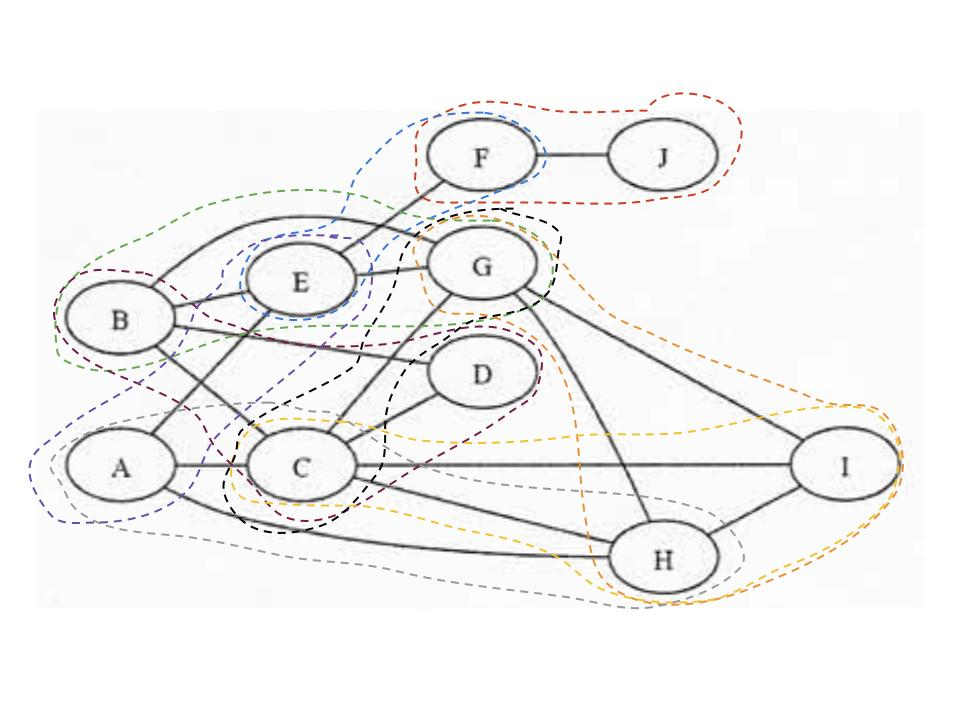
\includegraphics[width=8 cm]{Cliques.jpg}

\end{figure}

\begin{columns}
\column{3.5cm}
\begin{eqnarray}
&C_1:& F,J \nonumber\\
&C_2:& F,E \nonumber\\
&C_3:& B,E,G \nonumber
\end{eqnarray}
\column{3.5cm}
\begin{eqnarray}
&C_4:& G,H,I,C \nonumber\\
&C_6:& A,C,H \nonumber\\
&C_7:& B,C,D \nonumber
\end{eqnarray}
\column{3.5cm}
\begin{eqnarray}
&C_8:& A,E \nonumber\\
&C_9:& B,C,G \nonumber
\end{eqnarray}
\end{columns}
\end{frame}
%++++++++++++++++++++++++++++++++++++++++

%%%%%%%%%%%%%%%%%%%%%%%%%%%%%%%%%%%%%%%%%%%%%%%%%%%%%
\section*{11.2 Cliques and Seperators}

%++++++++++++++++++++++++++++++++++++++++
\begin{frame}
  \frametitle{a) construction of the moral graph}

\begin{figure}[h]
  \centering
  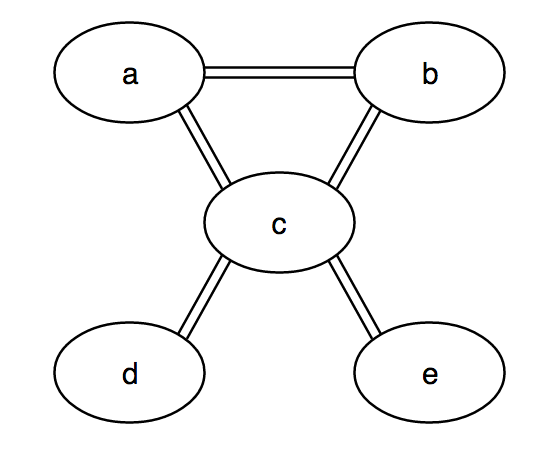
\includegraphics[width=6 cm]{moral_graph.png}
  \caption{moral graph of given DAG}
\end{figure}

\end{frame}
%++++++++++++++++++++++++++++++++++++++++
\begin{frame}
  \frametitle{b) pdf from cliques and seperators}

\begin{itemize}
\item we show that the DAG representation equals the given formula for the joint distribution:
\end{itemize}

\begin{eqnarray}
P(a,b,c,d,e) \;=\; P(a)P(b)P(c|a,b)P(d|c)P(e|c) \\
=\; \frac{P(a,b)P(a,b,c)P(d,c)P(e,c)}{P(c)^2P(a,b)} \\
=\; \frac{P(a,b,c)P(d,c)P(e,c)}{P(c)P(c)}\\
=\; \frac{P(C_1)P(C_2)P(C_3)}{P(S_1)P(S_2)}\;=\; \frac{\prod_i P(C_i)}{\prod_j P(S_j)} \\
\end{eqnarray}


\end{frame}
%++++++++++++++++++++++++++++++++++++++++

%%%%%%%%%%%%%%%%%%%%%%%%%%%%%%%%%%%%%%%%%%%%%%%%%%%%%
\section*{11.4 Potential Functions}

%++++++++++++++++++++++++++++++++++++++++
\begin{frame}
  \frametitle{a) potential functions and the clique-marginal representation}

\begin{itemize}
\item potential functions are used to represent joint probabilities of cliques, can be easily updated by new data
\item potential functions are strictly positive, real-valued and only depend on random variables in their assigned clique
\item don't need to be normalised so that $\psi_n(C_n) = \alpha\,P(C_n),\;\alpha>0$
\item link between joint probability distribution and clique-marginal representation:
\begin{equation}
P(V \in \mathcal{V})\;=\;\prod_{V \in \mathcal{V}} P(V|V_{pa(V)})\;=\;\frac{\prod_i P(C_i)}{\prod_j P(S_j)}\;=\; \alpha \frac{\prod_i \psi_i(C_i)}{\prod_j \psi_j(S_j)}
\end{equation}
\item at the beginning, all potentials are chosen to be 1
\end{itemize}


\end{frame}
%++++++++++++++++++++++++++++++++++++++++
\begin{frame}
  \frametitle{b) exploitation of potential functions to make inferences}
\begin{enumerate}
\item update clique potential
\begin{itemize}
  \item inference by observed evidence at one node: $V_l=v_l$
  \item introduce indicator function $E(V_l) = \begin{cases}
                                                  1 &\text{se $V_l = v_l$}\\
                                                  0 &\text{se else}
                                                  \end{cases}$
  \item update clique potential of observed node: $\psi_{i,new}(C_i)=\psi_{i}(C_i)E(V_l)$
\end{itemize}
\item message passing
\begin{itemize}
  \item new seperator potential: $ \psi_c^*(S_c)\;=\; \sum_{V \in C_i, V \notin \psi_c} \psi_i(V \in C_i) $
  \item the update of one clique demands updates of the neighbor cliques which happens by passing the update ratio $\frac{\psi_c^*(S_c)}{\psi_c(S_c)}$ ($S_c$: common seperator)
  \item updated neighbor potential obtained by multiplication of current potential with the update rate
\end{itemize}
\end{enumerate}
\end{frame}
%++++++++++++++++++++++++++++++++++++++++
\begin{frame}
  \frametitle{c) benefit in comparison to DAG factorisation}

\begin{itemize}
\item simpler and clearer models due to substitution of subgraphs by cliques
\item highly improved interference
\end{itemize}


\end{frame}
%++++++++++++++++++++++++++++++++++++++++

%%%%%%%%%%%%%%%%%%%%%%%%%%%%%%%%%%%%%%%%%%%%%%%%%%%%%%%%%%%%%%%%%%%
\begin{frame}
\frametitle{Literature}
\footnotesize{
\begin{thebibliography}{99}

\bibitem[1]{LN}'Machine Intelligence I', Lecture Notes by Prof. Dr. Klaus Obermayer, 2015

\bibitem[2]{Ch3}'Probabilistic Networks and Expert Systems', Chapter 3, Cowell et al., 1999

\end{thebibliography}}
\end{frame}

%%%%%%%%%%%%%%%%%%%%%%%%%%%%%%%%%%%%%%%%%%%%%%%%%%%%%%%%%%%%%%%%%%%

\end{document}
